A la hora de usar la función \ctexttt{tag} que sirve para etiquetar gramaticalmente las palabras de un \emph{string} notamos que los casos que sea una cadena sin significado se le asigna la etiqueta \ctexttt{'NN'}, que debería corresponder a un sustantivo. Veamos un ejemplo:
\begin{minted}{python}
import pattern.es
import random
import string

x= "danzar amigable barrilete asdfg"
print(pattern.es.tag(x, tokenize=True, encoding='utf-8'))

x = ''.join([random.choice(string.ascii_letters + string.digits) for n in range(32)])
print(pattern.es.tag(x, tokenize=True, encoding='utf-8'))
\end{minted}
Esto nos imprime:
\begin{cverbatim}
[('danzar', 'VB'), ('amigable', 'JJ'), ('barrilete', 'NN'), ('asdfg', 'NN')]
[('KD1mrZi6SwpZN25arEGv4TugHLAy2BYC', 'NN')]
\end{cverbatim}
Las primeras tres palabras las etiqueta correctamente como verbo, adjetivo y sustantivo, pero ya en la siguiente vemos algo raro. Sin encontrar documentación al respecto procedemos a revisar el repositorio
\href{https://github.com/clips/pattern/tree/master/pattern/text/es}{pattern.es} 
donde notamos el archivo
\href{https://github.com/clips/pattern/blob/master/pattern/text/es/es-spelling.txt}{es-spelling.txt}
, el cual tiene un diccionario gigantesco con palabras como clave y un valor numérico
por ejemplo \ctexttt{'ultravioleta': 5}. No se indica que significa el valor, entonces buscamos donde lo usa. En el archivo
\href{https://github.com/clips/pattern/blob/master/pattern/text/es/__init__.py}{\texttt{\_init\_\_.py}}
define la variable \href{https://github.com/clips/pattern/blob/5b85d998c30ddc6772b56310713530224466083a/pattern/text/es/__init__.py\#L222}{\ctexttt{spelling}}:

\begin{minted}{python}
spelling = Spelling(
        path = os.path.join(MODULE, "es-spelling.txt")
)
\end{minted}

que luego se usa para definir una 
\href{https://github.com/clips/pattern/blob/5b85d998c30ddc6772b56310713530224466083a/pattern/text/es/__init__.py\#L271}{función}
que sugiere correcciones. La clase
\href{https://github.com/clips/pattern/blob/5b85d998c30ddc6772b56310713530224466083a/pattern/text/es/__init__.py\#L44}{\ctexttt{Spelling}}
la importa de \href{https://github.com/clips/pattern/tree/master/pattern/text}{\texttt{pattern.text}}:
\begin{minted}{python}
# Import spelling base class.
from pattern.text import (
    Spelling
)
\end{minted}
En el
\href{https://github.com/clips/pattern/blob/master/pattern/text/__init__.py}{\texttt{\_\_init\_\_.py}} de \texttt{pattern.text} podemos investigar la
\href{https://github.com/clips/pattern/blob/5b85d998c30ddc6772b56310713530224466083a/pattern/text/__init__.py\#L2601}{clase}, dónde notamos el comentario:

\begin{minted}{python}
# Based on: Peter Norvig, "How to Write a Spelling Corrector", http://norvig.com/spell-correct.html
\end{minted}

Siguiendo el \href{http://norvig.com/spell-correct.html}{link}:

\begin{minted}{python}
WORDS = Counter(words(open('big.txt').read()))

def P(word, N=sum(WORDS.values())):
    "Probability of `word`."
    return WORDS[word] / N
\end{minted}

Podemos deducir que el \emph{diccionario} de 
\texttt{es-spelling.txt} es en realidad un
\href{https://docs.python.org/2/library/collections.html\#collections.Counter}{\emph{Counter}}. Por lo tanto el numerito de los \texttt{values()} es un contador de la cantidad de veces que apareció la palabra en el entrenamiento que tuvo el paquete, como decía al principio:

\begin{verbatim}
;;;   Based on several public domain books from Project Gutenberg
;;;   and Wikipedia articles and online Spanish newspaper articles.
\end{verbatim}

Otro archivo importante que se encuentra en \emph{pattern.es},  es el
\href{https://github.com/clips/pattern/blob/master/pattern/text/es/es-lexicon.txt}{\textbf{lexicon}}.
Es tan grande que el visor de github no lo carga y hay que verlo en
\href{https://raw.githubusercontent.com/clips/pattern/master/pattern/text/es/es-lexicon.txt}{\texttt{raw}}.
En el vemos que tiene palabras junto con lo que parece ser el \emph{part\_of\_speech\_}, por ej \ctexttt{ballet NCS}. Si buscamos la referencia
a \texttt{NCS}. en la
\href{https://www.clips.uantwerpen.be/pages/MBSP-tags}{lista de abreviaciones}
notamos que no aparece allí. Tampoco en ninguno de estos
\href{https://www.sketchengine.eu/tagsets/english-part-of-speech-tagset/}{\emph{tag
sets}}. El único resultado alegórico lo encontramos en éste
\href{https://www.aclweb.org/anthology/C14-1099}{paper} donde la sigla
hace referencia al termino en inglés \emph{Noun Compounds}, o sea 

#################################################################################

sustantivos compuestos, lo cual en mi opinión ballet no es pero bueno
sigamos mirando que más tiene \textbf{lexicon}

En el
\href{https://github.com/clips/pattern/blob/5b85d998c30ddc6772b56310713530224466083a/pattern/text/es/__init__.py\#L220}{\texttt{\_\_init\_\_.py}}
se usa:
\begin{minted}{python}
lexicon = parser.lexicon # Expose lexicon.
\end{minted}

Por lo tanto es otro atributo del paquete. Probamos en la linea de comandos que imprime lo siguiente:
\begin{Verbatim}[breaklines=true, breakanywhere=true]
    >>> import pattern.es
    >>> print(type(pattern.es.spelling))
    <class 'pattern.text.Spelling'>
    >>> print(dir(pattern.es.spelling))
    ['CYRILLIC', 'LATIN', '__class__', '__contains__', '__delattr__','__delitem__', '__dict__', '__dir__', '__doc__', '__eq__', '__format__', '__ge__', '__getattribute__', '__getitem__', '__gt__', '__hash__', '__init__', '__init_subclass__', '__iter__', '__le__', '__len__', '__lt__', '__module__', '__ne__', '__new__', '__reduce__', '__reduce_ex__', '__repr__','__setattr__', '__setitem__', '__sizeof__', '__str__', '__subclasshook__', '__weakref__', '_edit1', '_edit2', '_known','_lazy', '_path', 'alphabet', 'clear', 'copy', 'fromkeys', 'get', 'items', 'keys', 'language', 'load', 'path', 'pop', 'popitem', 'setdefault', 'suggest', 'train', 'update', 'values']
    >>>
\end{Verbatim}

Notamos que tiene el método \texttt{keys()}, lo mismo sucede con \texttt{pattern.es.lexicon}, entonces probamos este pequeño programa:
\begin{listing}
\begin{minted}{python}
import pattern.es
c = 0
for x in pattern.es.lexicon.keys():
	if not( x in pattern.es.spelling.keys() ):
		print(x, end=', ')
		c += 1
print("\n")
print('Cantidad de palabras en lexicon que NO estan en spelling: ',c)
\end{minted}
\end{listing}
El resultado de LISTING se puede er en la FIGURA
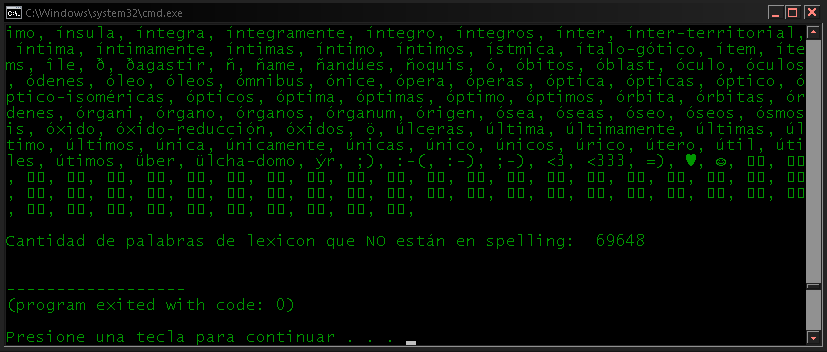
\includegraphics[width=\textwidth,keepaspectratio]{img/lexnspe.png}

Siguiendo con esa idea probamos con \texttt{spelling}:
\begin{minted}{python}
c = 0
for x in pattern.es.spelling.keys():
	if not( x in pattern.es.lexicon.keys() ):
		print(x, end=', ')
		c += 1
print("\n")
print('Cantidad de palabras de spelling que no estan en lexicon: ',c)
\end{minted}
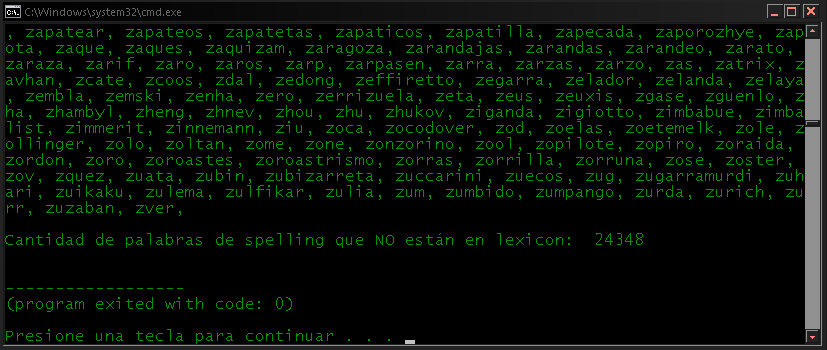
\includegraphics[width=\textwidth,keepaspectratio]{img/spenlex.png}
Y por último la intersección:
\begin{minted}{python}
c = 0
for x in pattern.es.spelling.keys():
	if x in pattern.es.lexicon.keys():
		print(x, end=', ')
		c += 1
print("\n")
print('Cantidad de palabras de spelling que TAMBIÉN están en lexicon: ',c)
\end{minted}

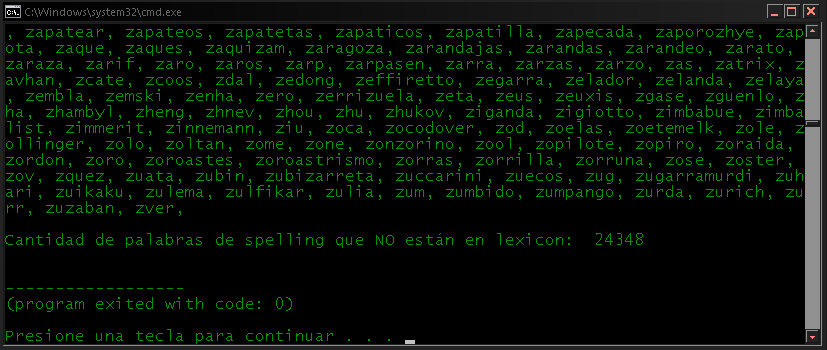
\includegraphics[width=\textwidth,height=0.8\textheight,keepaspectratio]{img/spenlex.png}

Como vemos son archivos disjuntos, lexicon tiene más símbolos,
pero spelling también tiene palabras en otros idiomas y casos extraños,
por ejemplo, no está `zanahoria' pero sí `zanahorias'.
Busquemos las entradas más largas de cada archivo:

\begin{minted}{python}
lista = list(pattern.es.spelling.keys())
mas_largo = max(lista, key=len)
print(mas_largo,' - ', len(mas_largo))
\end{minted}
Resulta:
\\\ctexttt{bienintencionadamente  -  21}
\\Con \texttt{lexicon} obtenemos:
\\\ctexttt{.......................................................................  -  71}

Si contamos los distintos valores del diccionario:
\begin{minted}{python}
from collections import Counter
c = Counter(pattern.es.lexicon.values())

print(c)
\end{minted}
Esto devuelve:
\begin{cverbatim}
Counter({'NP': 23462, 'NCS': 13780, 'AQ': 11017, 'VMI': 9016,
         'NCP': 7568, 'Z': 5969, 'VMP': 5259, 'VMN': 2206, 'RG': 1731,
         'VMS': 1485, 'VMG': 1258, 'NC': 1082, 'Zu': 441, 'W': 295,
         'VMM': 249, 'I': 161, 'Zp': 130, 'SP': 111, 'DI': 74, 'SYM': 63,
         'Zm': 59, 'AO': 56, 'VAI': 54, 'Fz': 48, 'PP': 42, 'DD': 29,
         'VSI': 27, 'Zd': 25, 'DP': 25, 'PI': 21, 'CC': 21,'PD': 20,
         'PR': 16, 'PT': 16, 'CS': 15, 'VAS': 15, 'DA': 13, 'VSS': 9,
         'Fs': 6, 'PX': 6, 'Fe': 4, 'Fc': 3, 'VAG': 3, 'VAN': 3, 'Fa': 2,
         '"': 2, 'Fg': 2, 'Fh': 2, 'Fr': 2, 'Fi': 2, 'DT': 2, 'RN': 2,
         'P0': 2, 'VSN': 2, 'VSG': 2, 'Fpa': 1, 'Fpt': 1, 'Fp': 1, 'Fd': 1,
         'Fx': 1, 'VSP': 1, 'Fl': 1})
\end{cverbatim}

Por lo que vuelve a surgir la duda de qué significaran esos \emph{tags}
ya que no se encuentran en la
\href{https://www.clips.uantwerpen.be/pages/MBSP-tags}{tabla}
proporcionada por pattern. Viendo la definición de
\href{https://www.clips.uantwerpen.be/pages/pattern-en}{\texttt{parse}}:

\begin{minted}{python}
parse(string,
   tokenize = True,         # Split punctuation marks from words?
       tags = True,         # Parse part-of-speech tags? (NN, JJ, ...)
     chunks = True,         # Parse chunks? (NP, VP, PNP, ...)
  relations = False,        # Parse chunk relations? (-SBJ, -OBJ, ...)
    lemmata = False,        # Parse lemmata? (ate => eat)
   encoding = 'utf-8'       # Input string encoding.
     tagset = None)         # Penn Treebank II (default) or UNIVERSAL.
\end{minted}

\texttt{UNIVERSAL} se refiere a ese otro tagset que vemos en
\textbf{lexicon}. Veamos qué palabras de ese conjunto no se corresponden con el etiquetado que proporciona la función \ctexttt{tag}. La mima recibe un \emph{string} como parámetro, lo separa en palabras y devuelve una lista con las tuplas \texttt{(palabra, etiqueta)}, (por eso accedemos con \ctexttt{[0][1]}):

\begin{minted}{python}
for x in lexicon:
	if lexicon[x] != tag(x, tokenize=True, encoding='utf-8', tagset = 'UNIVERSAL')[0][1]:
		print(x, end=', ')
\end{minted}

\begin{Verbatim}[breaklines=true, breakanywhere=true]
#11, #12-438-512, #12-439-610, #13, #136, #14, #15, #16, #19, #20, #21, #22, #228, #23, #24, #25, #26, #27, #28, #285, #29, #30, #31, #32, #33, #34, #344, #35, #36, #360, #361, #37, #38, #400, #42, #45, #50, #55, #61, #62, #63, #75, #83, #86, #89, #93, #94, #96, $1.99, $13, $150, $200, $29,00, $3,000, $300, $37,000,000.00, $380,9, $4.03, $49, $50, $507,933,000, $58.59, $6.79, $60, $600.000, $70.60, $785, $79, $924.9, $93,7, &fmt=18, &fmt=22, *100, *18, *1929, *1ª, +-120, +10, +100.000, +12, +15, +20, +20/-20, +22, +30, +300.000, +33, +34, +44, +80.000, ,1999, ,2002, ---, ----,-//W3C//DTD, -00198, -10, -1073, -1080, -1085, -11, -1150, -1160, -1190, -12, -1210, -1211, -1214, -1217, -1244, -1255, -1292, -13, -1347, -14, -15, -16, -1732, -1767, -1884, -1886, -1906, -1914, -1940, -20, -20º, -20ºC, -29, -30, -32, -320, -350, -40, -50, -67, -6º, -6ºC, -7º, -8ºC, ..., ...., ....., ......, ............................, ............................., ................................., ........................................., ............................................, .............................................., ................................................., ........................................................, ..................................................................., ......................................................................., .000, .000.000, .182, .256, .323, .346, .359, .380, .382, .385, .396, .401, .403, .412, .424, .438, .444, .446, .452, .464, .471, .477, .480, .483, .488, .494, .500, .514, .536, .542, .557, .585, .616, .750, .786, .7z, .824, .833, .848, .850, .853, .855, .856, .860, .892, 024.htm;, 4.php;, Col., EE.UU., Mar., Sto., Vols., arts., co., col., ed., id., id=242101545;, id=242101995;, ms., o.shtml;, pH., pl., pm., secret., vols., www.casadelaveiga.com;, www.cultura-sorda.eu;, www.difilm.com.ar),, www.distritodellama.com;, www.divinavoluntad.net;, www.el-guijo.es;, www.eurekared.com),, www.gesualdo.eu;, www.ibelieveinharveydent.com", www.kedainiai.info;, www.kedainiai.lt;, www.lfp.es;, www.mercedaragon.org;, www.mercedarios.cl;, www.mercedarios.com;, www.mercedarios.net;, www.mosovce.sk;, www.odemira.net;, www.samadegrado.es;, www.startalk.ch;,
\end{Verbatim}

Esto quiere decir que excepto esas cosas raras que están ahí, todo lo
demás son palabras que tienen su respectivo tag.
Concluimos entonces que para filtrar las palabras validas deberíamos buscar que esté en alguno de los dos conjuntos \emph{spelling} o \emph{lexicon} y, sí es así, lo se puede etiquetar con uno de los dos sistemas:

\begin{minted}{python}
from pattern.es import lexicon, spelling, tag

def clasificar(palabra):
	print(tag(palabra, tokenize=True, encoding='utf-8', tagset = 'UNIVERSAL'))
	print(tag(palabra, tokenize=True, encoding='utf-8'))

palabra = 'azucar'
if not palabra in spelling:
	if not palabra in lexicon:
		print('No se encuentra en pattern.es')
	else:
		print('La encontró en lexicon')
		clasificar(palabra)
else:
	print('La encontró en spelling')
	clasificar(palabra)
\end{minted}
Probamos distintas palabras:
\begin{cverbatim}
Camino
La encontró en lexicon
[('Camino', 'NCS')]
[('Camino', 'NN')]

camion
No se encuentra en pattern.es

camión
La encontró en lexicon
[('camión', 'NCS')]
[('camión', 'NN')]

vurro
No se encuentra en pattern.es

burro
La encontró en spelling
[('burro', 'NCS')]
[('burro', 'NN')]

Burro
No se encuentra en pattern.es

BURRO
No se encuentra en pattern.es

Argentina
La encontró en lexicon
[('Argentina', 'NP')]
[('Argentina', 'NNP')]

argentina
La encontró en spelling
[('argentina', 'AQ')]
[('argentina', 'JJ')]

ARGENTINA
No se encuentra en pattern.es
\end{cverbatim}

Falta perfeccionarlo, ya que algunos términos específicos no los encuentra y hay que filtrar las mayúsculas, no todas, ya que los \textbf{sustantivos propios} en lexicon están con mayúscula.

Además existe otra lista de palabras: \textbf{\texttt{verbs}} que tiene pocas palabras en relación a los otros, con lo cual sirve para buscar en ella primero que es más rápido. Sumando las funciones para capitalizar del modulo \ctexttt{string}:

\begin{minted}{python}
from pattern.es import verbs, tag, spelling, lexicon
import string
def clasificar(palabra):
	print( tag(palabra, tokenize=True, encoding='utf-8',tagset = 'UNIVERSAL'))
	print( tag(palabra, tokenize=True, encoding='utf-8'))
	print()


palabra = 'Camino'
print(palabra)
while palabra != 'q':
	if not palabra.lower() in verbs:
		if not palabra.lower() in spelling:
			if (not(palabra.lower() in lexicon) and not(palabra.upper() in lexicon) and not(palabra.capitalize() in lexicon)):
				print('No se encuentra en pattern.es')
			else:
				print('La encontró en lexicon')
				clasificar(palabra)
		else:
			print('La encontró en spelling')
			clasificar(palabra)
	else:
		print('La encontró en verbs')
		clasificar(palabra)
			
	print()
	palabra = input()
\end{minted}
Algunos ejemplos:
\begin{cverbatim}
BURRO
La encontró en spelling
[('BURRO', 'NCS')]
[('BURRO', 'NN')]

ArMoNíA
La encontró en lexicon
[('ArMoNíA', 'NCS')]
[('ArMoNíA', 'NN')]

BaILAr
La encontró en verbs
[('BaILAr', 'VMN')]
[('BaILAr', 'VB')]

djjd
No se encuentra en pattern.es
\end{cverbatim}